\documentclass[10pt,a4paper]{article}
\usepackage[utf8]{inputenc}
\usepackage{amsmath}
\usepackage{amsfonts}
\usepackage{amssymb}
\usepackage{pdfpages}
\usepackage{enumitem}
\author{Elvis Nava 870234 - Dario Ostuni 870321}
\title{Documentazione Tecnica\\
 Progetto Basi di Dati\\
\textit{DungeonAsDB - Comelico Simulator 2017}}
\date{Gennaio 2017}

\usepackage{listings}
\usepackage{color}

\definecolor{dkgreen}{rgb}{0,0.6,0}
\definecolor{gray}{rgb}{0.5,0.5,0.5}
\definecolor{mauve}{rgb}{0.58,0,0.82}

\lstset{frame=tb,
  language=python,
  aboveskip=3mm,
  belowskip=3mm,
  showstringspaces=false,
  columns=flexible,
  basicstyle={\small\ttfamily},
  numbers=none,
  numberstyle=\tiny\color{gray},
  keywordstyle=\color{blue},
  commentstyle=\color{dkgreen},
  stringstyle=\color{mauve},
  breaklines=true,
  breakatwhitespace=true,
  tabsize=3
}

\begin{document}

\maketitle

\textit{Comelico Simulator 2017} è un'applicazione web che consente a utenti registrati di partecipare a un gioco di ruolo di genere \textit{survival roguelike}, in cui si possono creare personaggi e con essi esplorare sedi universitarie abbandonate generate casualmente, combattere nemici di difficoltà crescente, trovare oggetti di diverse rarità e variazioni, e scambiarli con altri giocatori per valuta di gioco. I dati di gioco sono memorizzati in una base di dati e la logica di gioco è implementata completamente con procedure e trigger nel linguaggio procedurale della base di dati stessa.

Per l'implementazione sono stati scelti PostgreSQL come DBMS, PL/Python 3 come linguaggio procedurale e python come linguaggio per lo sviluppo dell'interfaccia web.

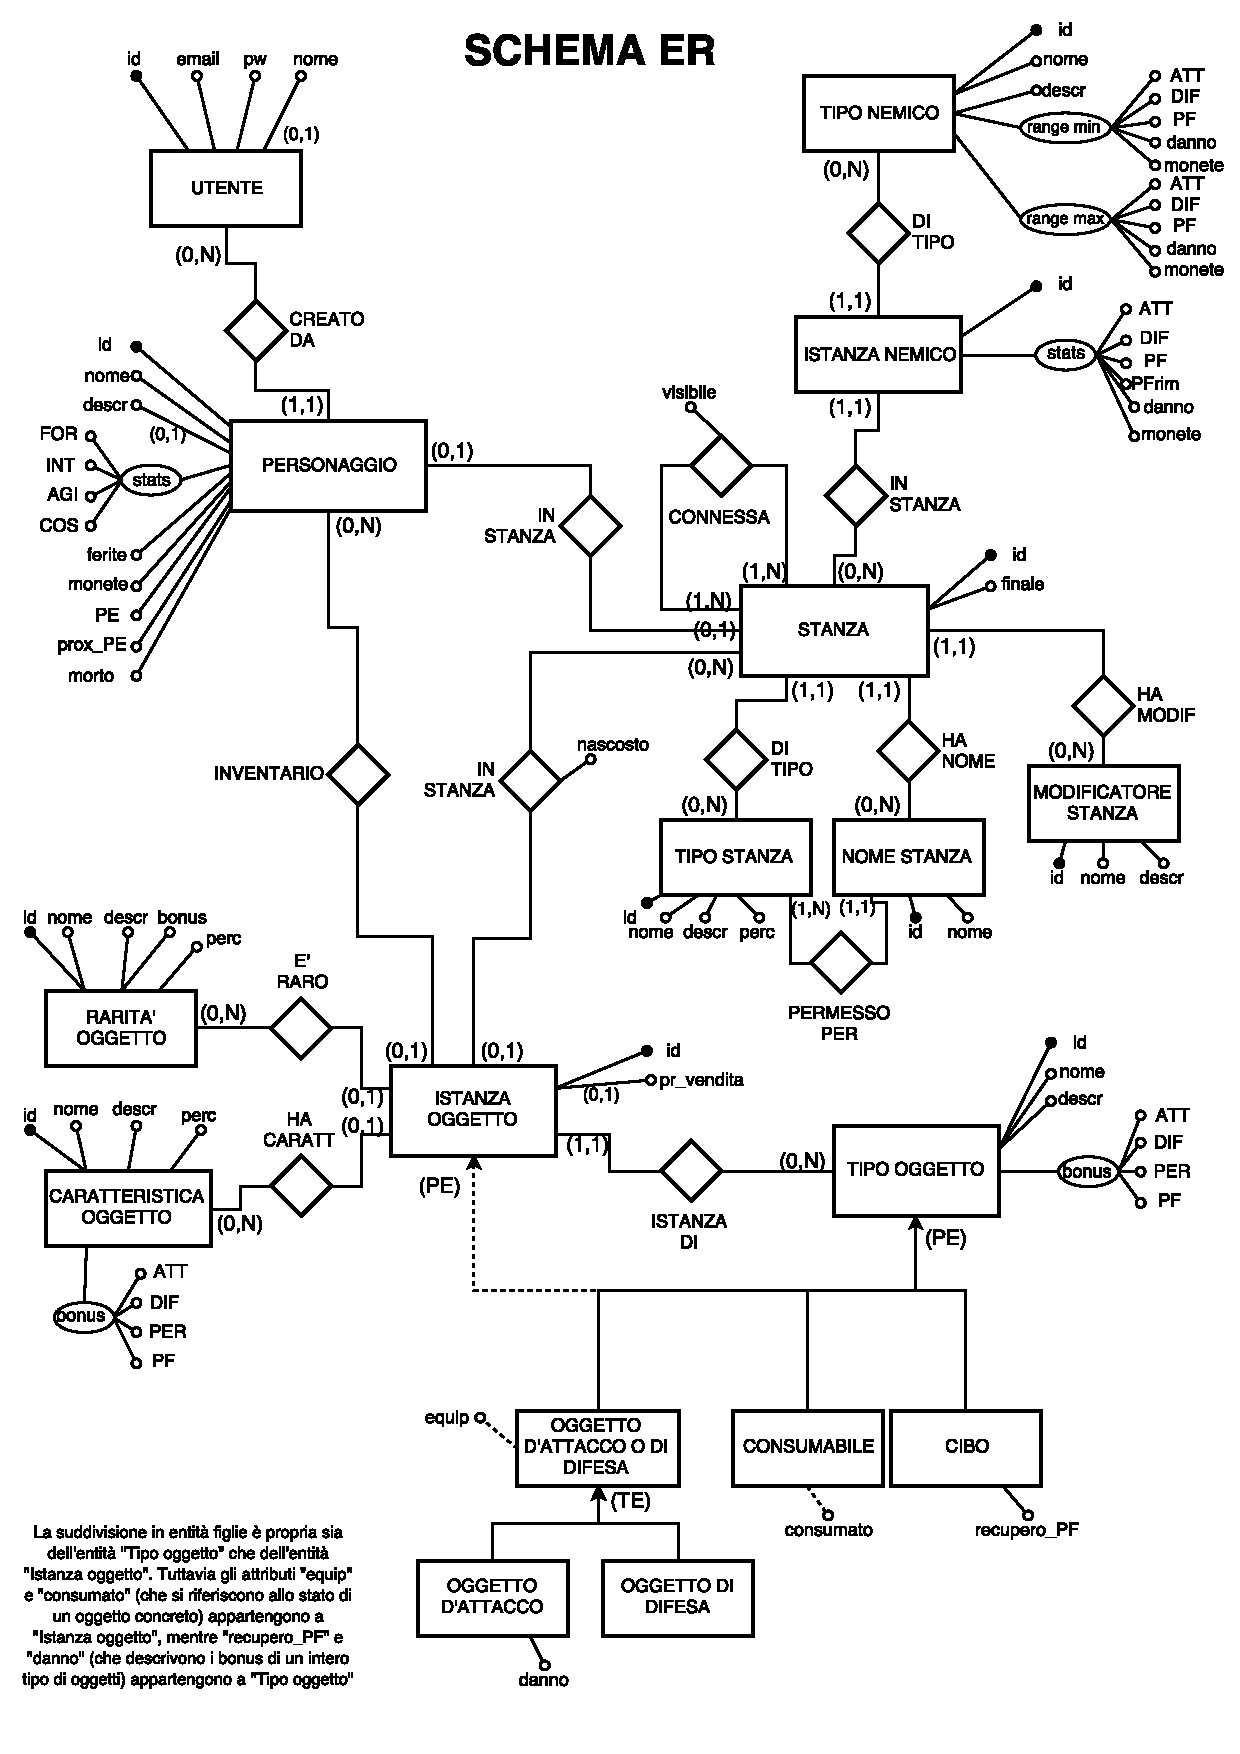
\includepdf{ER.pdf}

\section{Schema Concettuale ER della base di dati}
Concettualmente il Database è costituito dalle entità principali:

\subsection{Utente}
Rappresenta l'utente registrato all'applicazione, ha come attributi un id, i dati di login e un nome opzionale. È in grado di creare più Personaggi (relazione uno a molti).

\subsection{Personaggio}
Al centro dell'esperienza di gioco, è in relazione con diverse entità con cui può interagire. È creato da un Utente (relazione uno a molti), può trovarsi in una Stanza se la partita è cominciata (relazione uno a uno), ha un inventario di Oggetti (relazione uno a molti). Come attributi ha id, nome, descrizione opzionale, attributi base di gioco (FOR, INT, AGI, COS), contatore di ferite, di monete, Punti Esperienza (PE), PE accumulati nella partita corrente, e un flag per indicarne la morte. Tutti gli altri dati necessari per la gestione del Personaggio sono direttamente derivabili da questi o da attributi di entità con esso in relazione.

\subsection{Stanza}
Componente base per costruire dungeon, può ospitare un Personaggio (relazione uno a uno), può contenere Oggetti anche nascosti (relazione uno a molti), può contenere Nemici (relazione uno a molti), può essere connessa con un'altra Stanza attraverso un passaggio visibile o meno (relazione molti a molti). Come attributi propri dell'entità vi sono solo l'id e un flag per indicare se la stanza è finale (ovvero è possibile terminare l'avventura trovandosi in essa). Per il resto le differenti varietà di stanze generabili sono caratterizzate dalle relazioni (uno a molti) con Tipo Stanza per il nome e una descrizione generici, Nome Stanza per il nome proprio, e Modificatore Stanza per una descrizione aggiuntiva. Il Tipo Stanza ha anche un attributo contenente la percentuale di probabilità che sia scelto. Inoltre un Nome Stanza è permesso solamente per un certo Tipo (relazione uno a molti).

\subsection{Istanza e Tipo Nemico}
L'Istanza Nemico rappresenta un nemico concreto presente in una partita in corso, si trova in una Stanza (relazione uno a molti) e prende nome e descrizione dal suo Tipo (relazione uno a molti). I suoi attributi sono un id, i valori degli attributi di gioco con cui è stato generato (ATT, DIF, PF, danno), i Punti Ferita rimanenti (PFrim) e le monete che farà cadere alla morte.

Il Tipo Nemico rappresenta astrattamente un nemico possibilmente generabile dal gioco. I suoi attributi sono un id, un nome, una descrizione, il range per i valori possibili di ogni attributo di gioco del nemico (ATT, DIF, PF, danno) e per le monete fatte cadere alla morte.

\subsection{Istanza e Tipo Oggetto}
L'Istanza Oggetto rappresenta un oggetto concreto presente in un dungeon o nelle mani di un Personaggio. Può infatti trovarsi in una Stanza (relazione uno a molti) o alternativamente nell'inventario di un Personaggio (relazione uno a molti). Come attributi propri dell'entità vi sono solo l'id e un eventuale prezzo di vendita, nel caso l'oggetto sia stato messo in vendita nel mercato di gioco. Le diverse varietà di oggetti generabili sono caratterizzate dalle relazioni (uno a molti) con Tipo Oggetto per ottenere nome, descrizione e i bonus di base agli attributi (ATT, DIF, PER, PF), e facoltativamente con Caratteristica e/o Rarità Oggetto per ulteriori bonus. Caratteristica e Rarità Oggetto hanno ciascuna come attributi un nome, una descrizione e la percentuale di probabilità di essere selezionate durante la generazione. Caratteristica Oggetto ha anche valori dei bonus aggiuntivi differenti per ogni attributo, mentre Rarità Oggetto ha un bonus aggiuntivo unico per tutti gli attributi di gioco.

Tipo Oggetto, che rappresenta astrattamente un oggetto generabile dal gioco, fa inoltre parte di una gerarchia di generalizzazione Parziale Esclusiva con le entità figlie Consumabile, Cibo, e Oggetto d'Attacco/Difesa, a sua volta suddivisa con una gerarchia Totale Esclusiva nelle entità Oggetto d'Attacco e Oggetto di Difesa. Questa suddivisione è in realtà propria sia di Tipo Oggetto che di Istanza Oggetto: infatti i Consumabili hanno come attributo un flag per indicare se l'oggetto è stato consumato e gli Oggetti di Attacco/Difesa un flag per indicare se è stato equipaggiato, entrambi attributi di Istanze concrete di Oggetti, mentre il Cibo e gli Oggetti d'Attacco hanno come attributi rispettivamente il recupero di Punti Ferita e il danno inferto, entrambi attributi di Tipi astratti di Oggetti.

In particolare occorre notare come l'entità Cibo non sia stata progettata come sottoclasse di Consumabile. Infatti gli Oggetti dei due tipi funzionano in modo differente: mentre un'istanza di Cibo è cancellata al momento del consumo e il suo valore di recupero PF viene usato immediatamente per alleviare ferite, un'istanza di Consumabile è flaggata e viene cancellata solo dopo uno spostamento di stanza: il flag attiva i suoi valori di bonus ma allo stesso tempo nasconde la continuata presenza dell'oggetto al giocatore.

\newpage 

\section{Schema Relazionale della base di dati}
Lo schema ER è stato tradotto nel modello relazionale con le seguenti relazioni:
\begin{itemize}[leftmargin=*]
  \item[] UTENTE(\underline{id}, email, pw, nome*)
  \item[] PERSONAGGIO(\underline{id}, nome, descr*, \_FOR, \_INT, \_AGI, \_COS, monete, PE, prox\_PE, morto, \textit{creato\_da}, \textit{in\_stanza}*)
  \item[] STANZA(\underline{id}, finale, \textit{tipo}, \textit{nome}, \textit{modif})
  \item[] TIPO\_STANZA(\underline{id}, nome, descr, perc)
  \item[] NOME\_STANZA(\underline{id}, nome, \textit{permesso\_per})
  \item[] MODIF\_STANZA(\underline{id}, nome, descr)
  \item[] CONNESSA(\underline{\textit{stanza1}, \textit{stanza2}}, visibile)
  \item[] TIPO\_NEMICO(\underline{id}, nome, descr, min\_ATT, max\_ATT, min\_DIF, max\_DIF, min\_PF, max\_PF, min\_danno, max\_danno, min\_monete, max\_monete)
  \item[] IST\_NEMICO(\underline{id}, \_ATT, \_DIF, \_PFmax, \_PFrim, \_danno, monete, \textit{in\_stanza}, \textit{tipo})
  \item[] TIPO\_OGGETTO(\underline{id}, nome, \_ATT, \_DIF, \_PER, \_PF, \_danno*, classe*, recupero\_PF*)
  \item[] CAR\_OGGETTO(\underline{id}, nome, descr, add\_b\_ATT, add\_b\_DIF, add\_b\_PER, add\_b\_PF, perc)
  \item[] RARITA\_OGGETTO(\underline{id}, nome, descr, bonus, perc)
  \item[] IST\_OGGETTO(\underline{id}, \textit{di\_personaggio}, \textit{in\_stanza}, nascosto*, pr\_vendita*, equip*, consumato*, \textit{istanza\_di}, \textit{car}, \textit{rarita})
\end{itemize}

\subsection{Note sulla traduzione e sui controlli}
Le relazioni uno a molti dello schema ER sono state tradotte con l'inserimento di una chiave esterna nella tabella corrispondente all'entità con cardinalità massima 1. La relazione molti a molti tra stanze è stata tradotta con una tabella (CONNESSA) avente come chiave primaria una coppia di chiavi esterne riferite agli id delle stanze, con aggiunto l'attributo di relazione "visibile".

La gerarchia Parziale Esclusiva tra le classi di oggetti è stata tradotta conservando solamente l'entità padre, inserendo un attributo "classe" in TIPO\_OGGETTO   che può assumere i valori: "\_ATT" se l'oggetto è d'attacco, "\_DIF" se di difesa (l'ulteriore suddivisione Totale Esclusiva è stata precedentemente collassata mantenendo le sottoclassi), "cons" se è un consumabile, "cibo" se è cibo, o NULL (essendo la relazione parziale).

In TIPO\_OGGETTO si controlla con clausole CHECK che \_danno non sia NULL se la classe è "\_ATT" e sia NULL altrimenti, e che recupero\_PF non sia NULL se la classe è "cibo" e sia NULL altrimenti. Altri attributi che hanno a che fare con la classe dell'oggetto (eqip e consumato) sono tuttavia parte di IST\_OGGETTO, essendo proprietà di oggetti concreti. Il loro rispetto dei vincoli di classe non può quindi essere mantenuto con clasuole CHECK, ma viene controllato da trigger.

In IST\_OGGETTO sono inoltre specificati altri controlli: si controlla che almeno un attributo tra di\_personaggio e in\_stanza non sia NULL, e che non siano entrambi presenti contemporaneamente. Si controlla che pr\_vendita possa non essere NULL solamente quando di\_personaggio è specificato, e che nascosto possa non essere NULL solamente quando in\_stanza è specificato.

Su UTENTE si effettua il controllo del campo email, per assicurarsi che matchi il pattern '\%@\%.\%'.

\subsection{Domini, Viste e tabelle aggiuntive}
Per rappresentare certi dati sottoposti a vincoli sono stati aggiunti Domini aggiuntivi:
\begin{itemize}[leftmargin=*]
  \item[] \texttt{base\_bonus}: un valore intero tra -6 e +6 per i bonus di base (ATT, DIF, PER, PF, danno) dei tipi di oggetto.
  \item[] \texttt{main\_attribute}: un valore intero tra 3 e 18 per gli attributi di gioco base di un personaggio (FOR, INT, AGI, COS).
  \item[] \texttt{classe\_oggetto}: un valore di 4 caratteri compreso tra '\_ATT', '\_DIF', 'cons', e 'cibo'.
\end{itemize}
Sono state create diverse Viste per facilitare l'accesso ai dati:
\begin{itemize}[leftmargin=*]
  \item[] \texttt{stanza\_view}: effettua il join tra \texttt{tipo\_stanza}, \texttt{nome\_stanza} e \texttt{modif\_stanza}, selezionando tutti gli attributi necessari per avere la descrizione completa di una stanza.
  \item[] \texttt{ist\_nemico\_view}: effettua il join tra \texttt{ist\_nemico} e \texttt{tipo\_nemico} per recuperare il nome e la descrizione dell'istanza di un nemico (non seleziona i range per gli attributi, utili solo nella fase di generazione dell'istanza).
  \item[] \texttt{ist\_oggetto\_view}: effettua il join tra \texttt{ist\_oggetto}, \texttt{tipo\_oggetto}, \texttt{car\_oggetto} e \texttt{rarita\_oggetto}, selezionando tutti gli attributi necessari per caratterizzare l'istanza di un oggetto. In particolare somma i bonus base (soggetti a limite -6/+6) con eventuali bonus aggiuntivi dati dalla caratteristica e dalla rarità dell'oggetto. Una vista aggiuntiva \texttt{ist\_oggetto\_view\_no\_nasc} seleziona solo gli oggetti non nascosti.
  \item[] \texttt{personaggio\_attr\_deriv}: permette di ottenere gli attributi di gioco derivati (ATT, DIF, PER, PF massimi, PF rimanenti, danno) di un personaggio, calcolandoli a partire dai suoi attributi di gioco base e sommandoli ai bonus degli oggetti nel suo inventario (considerando oggetti di attacco o difesa solo se \texttt{equip}=true e oggetti consumati solo se \texttt{consumato}=true). I valori di bonus di inventario sono ottenuti con una subquery su \texttt{ist\_oggetto\_view} utilizzando l'operatore aggregato SUM sui bonus, raggruppando per personaggio.
\end{itemize}
Più tardi durante la progettazione dell'UI web è emersa la necessità di due tabelle aggiuntive:
\begin{itemize}[leftmargin=*]
  \item[] SESSIONE(\underline{chiave}, valore) per la memorizzazione delle sessioni degli utenti, avendo come "valore" un JSON contenente le variabili di python
  \item[] LANCIO\_DADI\_ATTR(\underline{\textit{utente}}, roll1, roll2, roll3, roll4, roll5) per memorizzare temporaneamente i lanci di dadi di un utente prima della creazione di un personaggio. Occorre memorizzare i valori poichè devono essere visualizzati nell'UI per essere scelti.
\end{itemize}

\section{Funzioni e Trigger}
Come linguaggio procedurale per la realizzazione di funzioni e trigger è stato scelto \texttt{plpython3}.

\subsection{Funzioni}

\subsubsection{\texttt{tira\_dadi\_attr(utente INTEGER) RETURNS void}}
Tira 5 volte 3d6 e salva i valori ottenuti nella tabella di lanci temporanei \texttt{lancio\_dadi\_attr}. Accetta come parametro \texttt{utente} l'id dell'utente che effettua il lancio e ritorna \texttt{void}.

\subsubsection{\texttt{crea\_personaggio(nome TEXT, descr TEXT, rolli\_for INTEGER, rolli\_int INTEGER, rolli\_agi INTEGER, rolli\_cos INTEGER, utente INTEGER) RETURNS void}}
Crea un nuovo personaggio utilizzando i dati forniti e i valori dei dadi della tabella \texttt{lancio\_dadi\_attr}. Il personaggio creato viene inserito in \texttt{personaggio}, vengono poi inseriti in \texttt{ist\_oggetto} i due oggetti iniziali per l'avventura (un oggetto d'attacco e una razione di cibo), segnandoli come di proprietà del personaggio. Accetta come parametri \texttt{nome} e \texttt{descr} il nome e la descrizione del personaggio, in \texttt{rolli\_for}, \texttt{rolli\_int}, \texttt{rolli\_agi}, \texttt{rolli\_cos} gli indici da 0 a 4 dei dadi scelti per i valori degli attributi base di gioco, e in \texttt{utente} l'id dell'utente creatore del personaggio. Ritorna \texttt{void}.

\subsubsection{\texttt{crea\_grafo() RETURNS INTEGER}}
Genera un grafo connesso di stanze per una nuova partita. Non prende parametri e ritorna l'id della stanza iniziale del dungeon.

Inizialmente vengono generate casualmente 32 stanze: viene deciso il \texttt{tipo\_stanza} con un confronto tra \texttt{random()} e il valore \texttt{perc} di percentuale di probabilità che questo venga scelto, poi si selezionano casualmente un \texttt{nome\_stanza} (tra quelli permessi per il tipo) e un \texttt{modif\_stanza}, controllando infine di volta in volta che una stanza totalmente uguale non sia già stata generata. Le stanze create sono inserite una di seguito nella tabella \texttt{stanza}, facendo sì che i loro id siano in sequenza.

Successivamente viene utilizzato questo algoritmo per generare  le connessioni e inserirle in \texttt{connessa}:
\begin{lstlisting}
mat_adj = [[0 for j in range(32)] for i in range(32)]

for i in range(16):
    a, b = randrange(32), randrange(32)
    if a == b:
        continue
    mat_adj[a][b] = 2
    mat_adj[b][a] = 2
for i in range(1, 32):
    to_node = randrange(i)
    mat_adj[i][to_node] = 1
    mat_adj[to_node][i] = 1

for i in range(32):
    for j in range(32):
        if mat_adj[i][j] != 0:
            visibile = True
            if mat_adj[i][j] == 2:
                visibile = False
            plan = plpy.prepare("INSERT INTO connessa VALUES($1, $2, $3)", ["integer", "integer", "boolean"])
            plpy.execute(plan, [i+start_node, j+start_node, visibile])
\end{lstlisting}
L'algoritmo, rappresentando il grafo con una matrice di adiacenza \texttt{mat\_adj}, genera prima alcuni passaggi casuali nascosti tra stanze (segnati nella matrice col valore 2), poi genera i passaggi restanti (segnati col valore 1) assicurandosi che il grafo sia connesso. Infine le connessioni sono inserite nella tabella, scorrendo la matrice e usando come id delle stanze gli indici i, j, sommati all'id della stanza iniziale (salvato precedentemente) \texttt{start\_node}.

\subsubsection{\texttt{inizia\_partita(id\_pers INTEGER) RETURNS void}}
Inizia una nuova partita chiamando \texttt{crea\_grafo()} per creare il dungeon, per poi popolarlo con oggetti e nemici di forza adatta al personaggio (prima controlla che il personaggio non si trovi già in una stanza e che non sia morto). Prende come parametro \texttt{id\_pers} l'id del personaggio e ritorna \texttt{void}.

Prima di tutto viene ottenuto un valore \texttt{difficulty} dato dalla somma degli attributi derivati del personaggio (ATT, DIF, PER, PF), poi si esegue un ciclo sulle stanze del dungeon (dalla prima alla finale in ordine per id) ottenendo ogni volta un valore \texttt{room\_difficulty} che parte da \texttt{difficulty} e aumenta fino a raddoppiare.

La presenza di nemici è decisa casualmente per tutte le stanze (tranne la prima e la finale) utilizzando una distribuzione geometrica di parametro 1/2 (ottenendo una media di 2 nemici per stanza). Un \texttt{tipo\_nemico} è scelto di volta in volta con probabilità $\frac{1}{3}^{\frac{\texttt{difficulty\_nemico}}{\texttt{room\_difficulty}}}$, usando come \texttt{difficulty\_nemico} la somma dei suoi attributi medi.

Gli oggetti sono generati in modo simile con una distribuzione geometrica di parametro 1/3 (ottenendo una media di 3 oggetti per stanza). Per la scelta del \texttt{tipo\_oggetto} si effettua inizialmente un confronto tra \texttt{random()} e 0.3 per decidere se considerare i tipi di classe "cibo" o gli altri (così da alzare artificialmente il numero di oggetti "cibo" generati), poi si genera un determinato oggetto con probabilità $\frac{1}{3}^{\frac{5*\texttt{livello\_tipo}}{\texttt{room\_difficulty}}}$, usando come \texttt{livello\_tipo} la somma dei bonus di base conferiti dal tipo di oggetto. Si scelgono a caso una \texttt{caratteristica\_oggetto} e una \texttt{rarita\_oggetto}, e si decide se includerle o meno nell'oggetto generato con un confronto di \texttt{random()} con il rispettivo valore del campo \texttt{perc}.

\subsubsection{\texttt{finisci\_partita(id\_pers INTEGER) RETURNS void}}
Controlla che il personaggio si trovi in una stanza finale, poi somma ai suoi \texttt{PE} (Punti Esperienza) i punti \texttt{prox\_PE} accumulati durante la partita, lo toglie dalla stanza in cui si trova settando \texttt{in\_stanza} a NULL e cancella le 32 stanze del dungeon all'indietro a partire da quella in cui si trova (gli id delle stanza erano tutti sequenziali). Accetta come parametro \texttt{id\_pers} l'id del personaggio e ritorna void.

\subsubsection{\texttt{mangia(id\_personaggio INTEGER, id\_ogg INTEGER) RETURNS void}}
Accetta come parametro \texttt{id\_personaggio} l'id del personaggio, come \texttt{id\_ogg} l'id dell'istanza oggetto "cibo" da mangiare. Se l'oggetto è in possesso del personaggio e si tratta effettivamente di un oggetto di classe "cibo", l'oggetto è eliminato e le \texttt{ferite} del personaggio sono ridotte di una quantità corrispondente al \texttt{recupero\_PF} fornito dal cibo. Ritorna void.

\subsubsection{\texttt{cerca\_segreti(id\_pers INTEGER) RETURNS void}}
Permette di rivelare connessioni tra stanze o oggetti nascosti spendendo 1 Punto Ferita. Accetta come parametro \texttt{id\_pers} e ritorna void. Le \texttt{ferite} del personaggio sono aumentate di 1 e si effettua un tiro di dado virtuale 1d20 confrontato con il valore di percezione \texttt{\_per} del personaggio. Se il tiro ha successo e il numero di oggetti e di passaggi nascosti è superiore a 0, allora si seleziona casualmente qualcosa da rivelare e la si rivela, rispettivamente settando \texttt{nascosto} a false o \texttt{visibile} a true. Eventuali nemici attaccano, viene quindi chiamata la funzione \texttt{attacco\_nemici}.

\subsubsection{\texttt{raccogli\_oggetto(id\_pers INTEGER, id\_ogg INTEGER) RETURNS void}}
Permette a un personaggio di raccogliere un oggetto, controllando che l'oggetto si trovi nella stessa stanza del personaggio e che non sia nascosto, settando inoltre \texttt{nascosto} a NULL al momento del raccoglimento. Accetta come parametri \texttt{id\_pers} l'id del personaggio e \texttt{id\_ogg} l'id dell'oggetto da raccogliere, ritorna void.

\subsubsection{\texttt{drop\_oggetto(id\_pers INTEGER, id\_ogg INTEGER) RETURNS void}}
Permette a un personaggio di far cadere a terra un oggetto, controllando che l'oggetto sia di proprietà del personaggio e settando \texttt{nascosto} a false al momento del drop. Accetta come parametri \texttt{id\_pers} l'id del personaggio e \texttt{id\_ogg} l'id dell'oggetto, ritorna void.

\subsubsection{\texttt{rolla\_attacco(\_att INTEGER, \_danno INTEGER, \_dif INTEGER) RETURNS INTEGER}}
Accetta come parametri \texttt{\_att} e \texttt{\_danno} il valore di attacco e danno dell'attaccante, e come \texttt{\_dif} il valore di difesa del difensore. Ritorna  \texttt{\_danno} se il tiro di un dado 1d20 sommato a (\texttt{\_att} + \texttt{\_dif}) supera 12, altrimenti ritorna 0.

\subsubsection{\texttt{attacco\_nemici(id\_pers INTEGER, id\_stanza INTEGER) RETURNS void}}
Effettua gli attacchi dei nemici contro il personaggio. Viene chiamata quando si svolgono azioni come attaccare, spostarsi, raccogliere, cercare. Non fa altro che chiamare \texttt{rolla\_attacco} per ogni nemico presente nella stanza del giocatore e con il valore restituito aumentare le \texttt{ferite} di quest'ultimo. Accetta come parametro \texttt{id\_pers} l'id del personaggio e come \texttt{id\_stanza} l'id della stanza in cui si trova. Ritorna void.

\subsubsection{\texttt{attacca(id\_pers INTEGER, id\_nemico INTEGER) RETURNS void}}
Permette di attaccare un nemico. Inizialmente controlla che il nemico non si trovi in una stanza diversa dal personaggio, poi chiama \texttt{attacco\_nemici} per far subire al personaggio gli attacchi dei nemici, e infine attacca il nemico: chiama \texttt{rolla\_attacco} e sottrae il valore di ritorno ai \texttt{\_PFrim} del nemico. Se questi scendono sotto lo 0 il nemico viene eliminato e alle \texttt{monete} e ai \texttt{prox\_PE} del personaggio vengono aggiunti rispettivamente le \texttt{monete} del nemico e il valore della somma dei suoi attributi. Accetta come parametri \texttt{id\_pers} l'id del personaggio e \texttt{id\_nemico} l'id del nemico attaccato. Ritorna void.

\subsubsection{\texttt{compra(id\_pers\_buyer INTEGER, id\_ogg INTEGER) RETURNS void}}
Compra un oggetto messo in vendita: controlla se l'oggetto è effettivamente in vendita (\texttt{pr\_vendita} non è NULL) e se il personaggio dispone di \texttt{monete} sufficienti, poi effettua la transazione. Per garantire il corretto trasferimento dell'oggetto e dei fondi viene utilizzata una subtransazione, implementata con il comando \texttt{plpy.subtransaction()} di PL/Python. La funzione accetta come parametri \texttt{id\_pers\_buyer} l'id del personaggio compratore e \texttt{id\_ogg} l'id dell'oggetto da comprare. Ritorna void.

\subsubsection{\texttt{vendi(id\_pers INTEGER, id\_ogg INTEGER, prezzo INTEGER) RETURNS void}}
Mette in vendita un oggetto dall'inventario di un personaggio: inizialmente controlla che l'oggetto sia di proprietà del personaggio, poi lo mette in vendita ponendo \texttt{pr\_vendita} uguale al prezzo, settando eventualmente anche \texttt{equip} a false. Accetta come parametri \texttt{id\_pers} l'id del personaggio, \texttt{id\_ogg} l'id dell'oggetto, e \texttt{prezzo} il prezzo di vendita. Ritorna void.

\subsubsection{\texttt{zaino(id\_personaggio INTEGER) RETURNS SETOF ist\_oggetto\_view}}
Funzione che a partire dalla vista \texttt{ist\_oggetto\_view} permette di ottenere un elenco degli oggetti visibili (non in vendita e non consumati) nello zaino di un personaggio. Accetta come parametro \texttt{id\_personaggio} l'id del personaggio di cui visualizzare lo zaino, ritorna un sottoinsieme di \texttt{ist\_oggetto\_view} composto dagli oggetti nello zaino.

\subsection{Trigger}
\subsubsection{\texttt{trigger\_capacita\_zaino BEFORE UPDATE OR INSERT ON ist\_oggetto FOR EACH ROW EXECUTE PROCEDURE funzione\_capacita\_zaino()}}
Controlla che il numero di oggetti nello zaino di un personaggio non superi ceil(\texttt{\_cos}/2). Per farlo chiama \texttt{zaino(id\_personaggio)} e usa l'operatore aggregato COUNT. Se il limite viene superato l'operazione è annullata e l'oggetto non viene raccolto.

\subsubsection{\texttt{trigger\_new\_att\_dif BEFORE INSERT ON ist\_oggetto FOR EACH ROW EXECUTE PROCEDURE funzione\_new\_att\_dif()}}
Controlla che istanze di oggetti di attacco o difesa siano creati con attributo \texttt{equip} non NULL e viceversa per gli altri oggetti, e controllo che oggetti consumabili siano creati con attributo \texttt{consumato} non NULL e viceversa per gli altri oggetti. Se viene rilevato un inserimento errato si modifica il campo inserendo NULL o false, in base alla classe del tipo di oggetto.

\subsubsection{\texttt{trigger\_equip\_att\_dif BEFORE UPDATE OR INSERT ON ist\_oggetto FOR EACH ROW EXECUTE PROCEDURE funzione\_equip\_att\_dif()}}
Controlla che un personaggio non possa equipaggiare contemporaneamente due oggetti di attacco o difesa. Se prova a equipaggiarne uno, setta \texttt{equip}=false a tutti gli altri oggetti del personaggio della stessa classe di quello equipaggiato.

\subsubsection{\texttt{trigger\_consum\_wearoff AFTER UPDATE ON personaggio FOR EACH ROW EXECUTE PROCEDURE funzione\_consum\_wearoff()}}
Se viene rilevato un cambiamento di stanza del personaggio (campo \texttt{in\_stanza}), vengono cancellati tutti gli oggetti del personaggio con l'attributo \texttt{consumato}=true. Così facendo si eliminano definitivamente gli oggetti consumati dal personaggio nella stanza, che pur essendo diventuti a lui invisibili fornivano bonus.

\subsubsection{\texttt{trigger\_check\_cambio\_stanza BEFORE UPDATE ON personaggio FOR EACH ROW EXECUTE PROCEDURE funzione\_check\_cambio\_stanza()}}
Controlla che gli spostamenti del personaggio da una stanza all'altra siano permessi, ovvero verifica che sia presente un collegamento tra le stanze nella tabella \texttt{connessa} e che \texttt{visibile}=true. Se le condizioni non sono verificate annulla l'azione.

\subsubsection{\texttt{trigger\_attacco\_cambio\_stanza AFTER UPDATE ON personaggio FOR EACH ROW EXECUTE PROCEDURE funzione\_attacco\_cambio\_stanza()}}
Quando il personaggio cambia stanza viene chiamata la funzione \texttt{attacco\_nemici (id\_personaggio, id\_stanza)} (usando come \texttt{id\_stanza} l'id della stanza precedente). Il personaggio viene quindi attaccato dai nemici in una stanza se si sposta da essa prima di averli eliminati tutti.

\subsubsection{\texttt{trigger\_attacco\_raccogli\_oggetto AFTER UPDATE ON ist\_oggetto FOR EACH ROW EXECUTE PROCEDURE funzione\_attacco\_raccogli\_oggetto()}}
Quando il personaggio raccoglie un oggetto viene chiamata la funzione \texttt{attacco\_nemici (id\_personaggio, id\_stanza)}. Il personaggio viene quindi attaccato dai nemici in una stanza se raccoglie un oggetto prima di averli eliminati tutti.

\subsubsection{\texttt{trigger\_item\_drop\_morte AFTER UPDATE ON ist\_oggetto FOR EACH ROW EXECUTE PROCEDURE funzione\_morte()}}
\subsubsection{\texttt{trigger\_ferite\_morte AFTER UPDATE ON personaggio FOR EACH ROW EXECUTE PROCEDURE funzione\_morte()}}
Entrambi i trigger utilizzano la funzione \texttt{funzione\_morte()} per controllare la morte del personaggio rispettivamente dopo il raccoglimento o il drop di un oggetto (posso raccogliere un oggetto con bonus PF negativo e morire, o far cadere un oggetto che con il bonus PF teneva in vita il personaggio), e dopo il cambiamento del valore di \texttt{ferite} del personaggio. Se il valore \texttt{PF\_rim} dei Punti Ferita rimanenti ottenuto da \texttt{personaggio\_attr\_deriv} è inferiore o uguale a 0, allora viene settato l'attributo \texttt{morto}=true. Viene poi cancellato il dungeon in cui il personaggio si trovava cancellando le stanze scorrendole per id all'indietro fino a trovare una stanza finale (da non cancellare), e in avanti fino a trovare una stanza finale (da cancellare). Vengono anche cancellati da \texttt{ist\_oggetto} tutti gli oggetti di proprietà del personaggio, questo perchè a differenza di quando si termina una partita con una vittoria, la morte impedisce permanentemente al personaggio di ricominciare nuove partite.

\newpage 

\section{Web UI}
L'interfaccia di gioco è implementata in \texttt{python3} utilizzando CGI (Common Gateway Interface) per generare dinamicamente pagine in XHTML5. Per la connessione con PostgreSQL viene usato il connettore \texttt{psycopg2}.

\subsection{\texttt{index.py}}
\texttt{index.py} è suddiviso in una parte di inizializzazione e una di generazione delle pagine.

Inizialmente si connette al database, fa il parsing dei cookie, inizializza o riprende la sessione dell'utente, dopodichè controlla che l'utente abbia i permessi per visitare la pagina.

In base all'argomento GET \texttt{page} vengono stampate pagine differenti, corrispondenti a ogni fase di gioco.

Alla fine chiude la sessione, fa il commit su database della transazione e stampa la pagina.

\subsection{Classi ausiliarie}
Sono state implementate diverse classi ausiliarie per modularizzare il programma:
La classe \texttt{Page} ha lo scopo di facilitare la generazione del codice XHTML5 tramite chiamate di metodi. La classe \texttt{DB} è un'interfaccia con il controllo degli errori di \texttt{psycopg2}. La classe \texttt{Session} gestisce la sessione degli utenti facendo richieste alla tabella \texttt{sessione} del database.

\end{document}